\section{Results}
In this section we present results of runing the simulation described in the previous section. The subsections below focus on the following research questions, 

\begin{itemize}
  \item How well does the RFEA derived ion energy distribution function represents the actual energy distribution function of ions at the bounding electrode (i.e., at G$_0$)? 
  \item What is the effect of ion space charge inside the RFEA on the space potential and electric field?  
  \item What is the effect of different spacings between grids on the RFEA derived ion energy distribution function when compared to the actual one at the bounding electrode?
\end{itemize}


\subsection{Ion energy distribution profile}
Fisrt, we run the simulation at various pressures and compared the derived ion energy disribution function with the actual energy distribution as recorded in the model at G$_0$. The RFEA configuration is as follows: 2332 stack, G$_1$=C=-60~V, G$_3$=-70~V, grid transparency 100~\%. The plasma sheath potential used is AC with maximum voltage difference across the sheath of 2000~V (i.e., V$_\text{pk-pk}$), the radio-frequency 13.56~MHz, and the plasma density $10^{16}$~m$^{-3}$. The pressure settings are 0.5, 1.0, 2.0, 5.0, 7.5 and 10.0~Pa. The model is run sweeping grid G$_2$ voltage setting from 0 to 1500~V in steps of 25~V. The number of ions whose trajectory is simulated per G$_2$ voltage step is 25000. The starting time for each ion is randomized uniformly across the radio-frequency period to represent that ions may enter the sheath at any point during the RF cycle. Each ion trajectory is followed for a total time of 1~$\mu$s. 

Figure~\ref{fig:IVcurve} shows the characteristic current-voltage curve for each model RFEA scan. The vertical axis is the ion count at the collector position. The ion count drops as the pressure is increased. 

\begin{figure}[htbp]
\centering
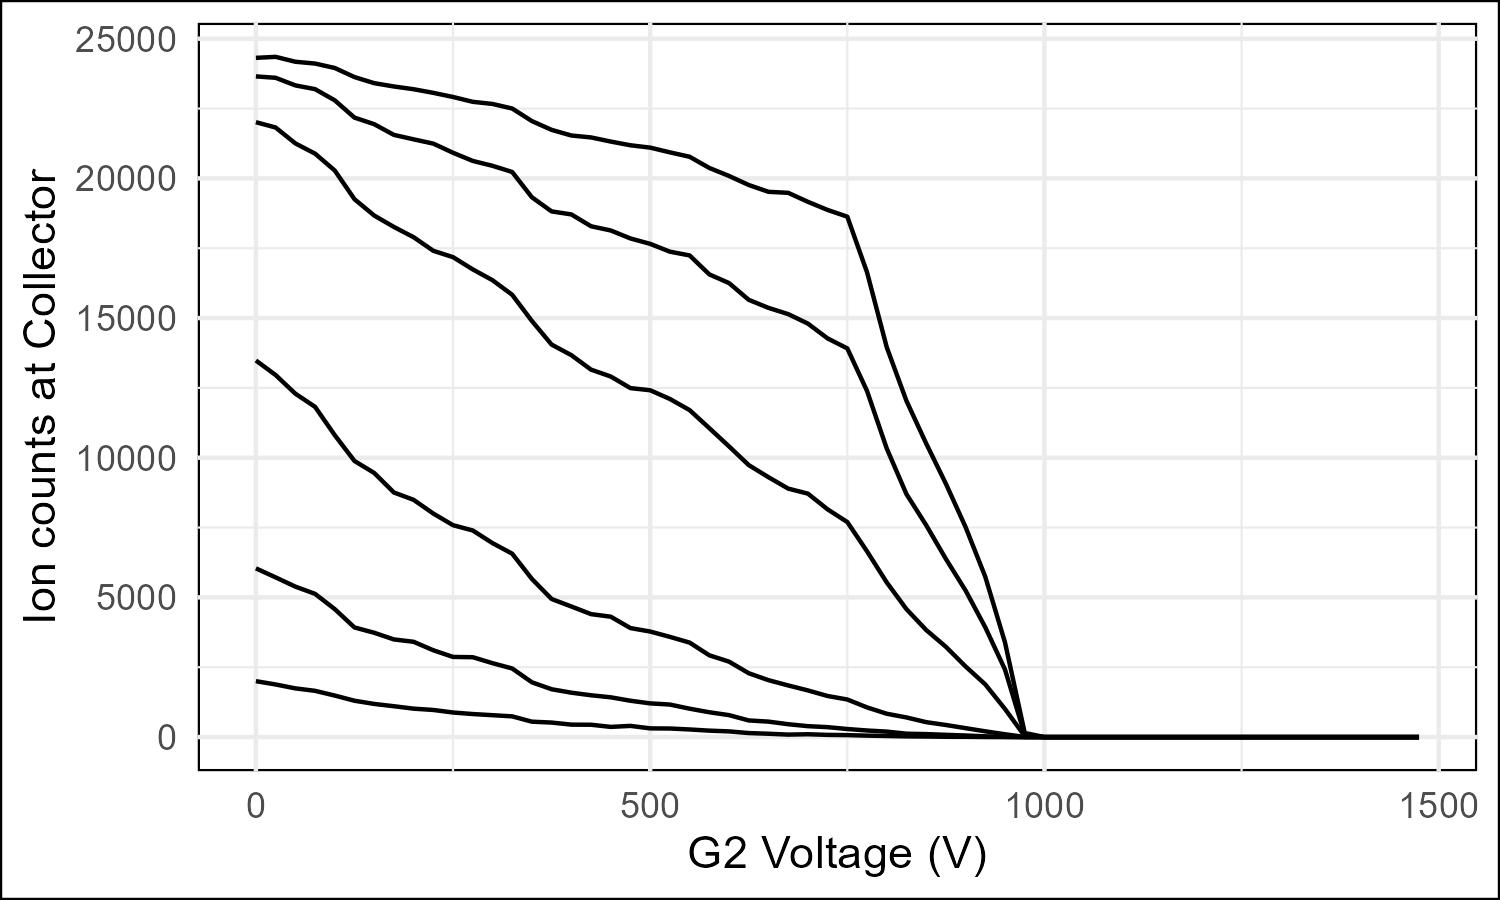
\includegraphics[width=0.45\textwidth]{Figures/IVcurve.jpeg}
\caption{Current-voltage characteristic curves where the current is represented by the ion count collected at the collector position. The curves from highest ion count value to lowest correspond to pressure settings from 0.5 to 10.0~Pa.}
\label{fig:IVcurve}
\end{figure}

The first derivative of the ion current is proportional to the ion energy distribution function~\cite{Hutchinson1987}. The set of curves on the left of Figure~\ref{fig:PressureScan} shows the first derivative of the curves in Figure~\ref{fig:IVcurve}. The derivatives are normalized and plotted with an offset in the vertical axis from lowest pressure setting at the top to highest pressure setting at the bottom. The ion energy distributions derived from the ion counts at the collector in the simulated RFEA for the various pressure settings can be contrasted with the actual ion energy distributions recorded at G$_0$, before the ions transport through the RFEA. These IEDFs are shown on the right of Figure~\ref{fig:PressureScan}. These scan was repeated using a smaller integration time step for the ion trajectories, $dt=10$~ps, to assess any potential artifact introduced in the simulation by the trajectory integration method, and no substantial qualitative difference on the energy distribution functions was observed (not shown). The derived IEDF at the collector exhibits more noise than the IEDF at G$_0$ due to the nature of the numerical derivative of the collector ion count; i.e., numerical derivatives of any parameter always ampiflies the parameter's noise. Here, a centered finite difference method was used to differentiate the Collector ion counts. All curves are shown without any smoothing. Still, both distributions show similar features, which is expected as ion-neutral collisions can not affect the shape of the ion energy distribution function~\cite{Baloniak2010}.   

\begin{figure}[htbp]
\centering
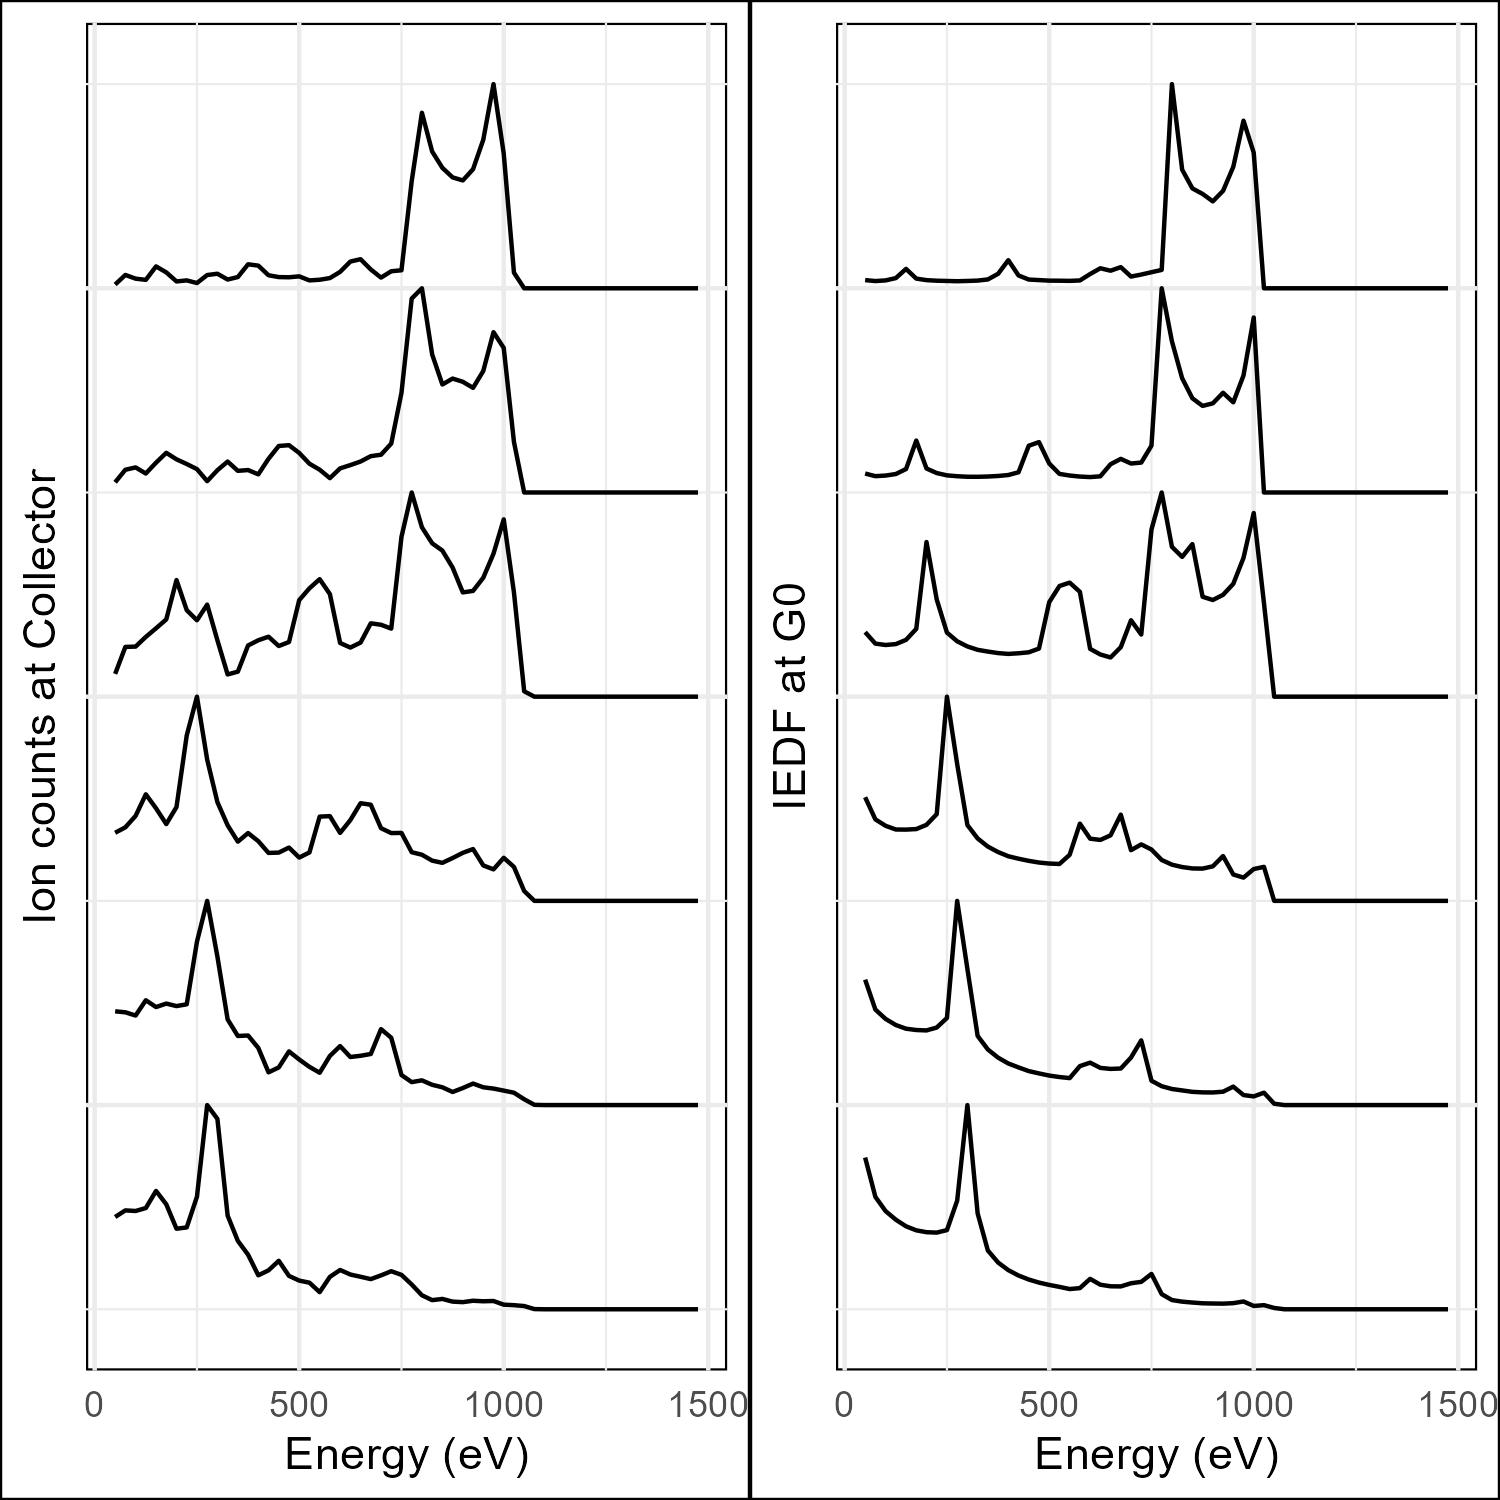
\includegraphics[width=0.45\textwidth]{Figures/PressureScan.jpeg}
\caption{Ion energy distribution functions. Left: First derivative of the current-voltage characteristic curves of Figure~\ref{fig:IVcurve}. Right: Plot of the ion energy distribution as recorded in the simulation at G$_0$, before ion transport through the RFEA. Both set of curves are normalized. The curves from top to bottom correspond to pressure settings from 0.5 to 10.0~Pa.}
\label{fig:PressureScan}
\end{figure}

The ion energy distributions of Figure~\ref{fig:PressureScan} exhibit a series of peaks which are the result of the oscillating plasma sheath and ion collisions with the background gas. More specifically, the sheath modulation, i.e., the time varying sheath edge and sheath electric field, can shape specific features of the IEDFs~\cite{Wild1989,Wild1991}. 




Second, we run the simulation at various radio-frequencies and compared the derived ion energy disribution function with the actual energy distribution as recorded in the model at G$_0$. The RFEA configuration is the same as the previous scan including the sheath potential maximum voltage difference 2000~V (i.e., V$_\text{pk-pk}$), the plasma density $10^{16}$~m$^{-3}$, and fixed pressure setting of 0.5~Pa. The model is run sweeping grid G$_2$ voltage setting from 0 to 1750~V in steps of 25~V. The number of ions whose trajectory is simulated per G$_2$ voltage step is 25000. The starting time for each ion is randomized uniformly across the radio-frequency period and each ion trajectory is followed for a total time of 1~$\mu$s. 

Figure~\ref{fig:IVcurve_FrequencyScan} shows the characteristic current-voltage curve for each model RFEA radio-frequency scan. The vertical axis is the ion count at the collector position. The set of curves on the left of Figure~\ref{fig:FrequencyScan} show the first derivative of the curves in Figure~\ref{fig:IVcurve_FrequencyScan}. The derivatives are normalized and plotted with an offset in the vertical axis from lowest radio-frequency setting at the top to highest at the bottom. The IEDFs recorded at G$_0$ are shown on the right of Figure~\ref{fig:FrequencyScan}. The distribution functions show a wider energy gap (between the lower energy peak to the higher energy peak) as the radio-frequency driving the sheath is reduced~\cite{Lieberman2005}. The lower frequencies have a stronger modulation effect on ions in transit through the sheath. However, there is no shift in the average of the energy peaks (mid point between the two peaks) as reported by Gahan et al.~\cite{Gahan2008}. Moreover, everything else being equal, as the radio-frequency is increased the maximum ion energy is approximately half the maximum voltage across the sheath; i.e., at 27.12~MHz, a 2~kV$_{pk-pk}$ sheath modulation accelerates ions up to approximately 1~keV.  

\begin{figure}[htbp]
\centering
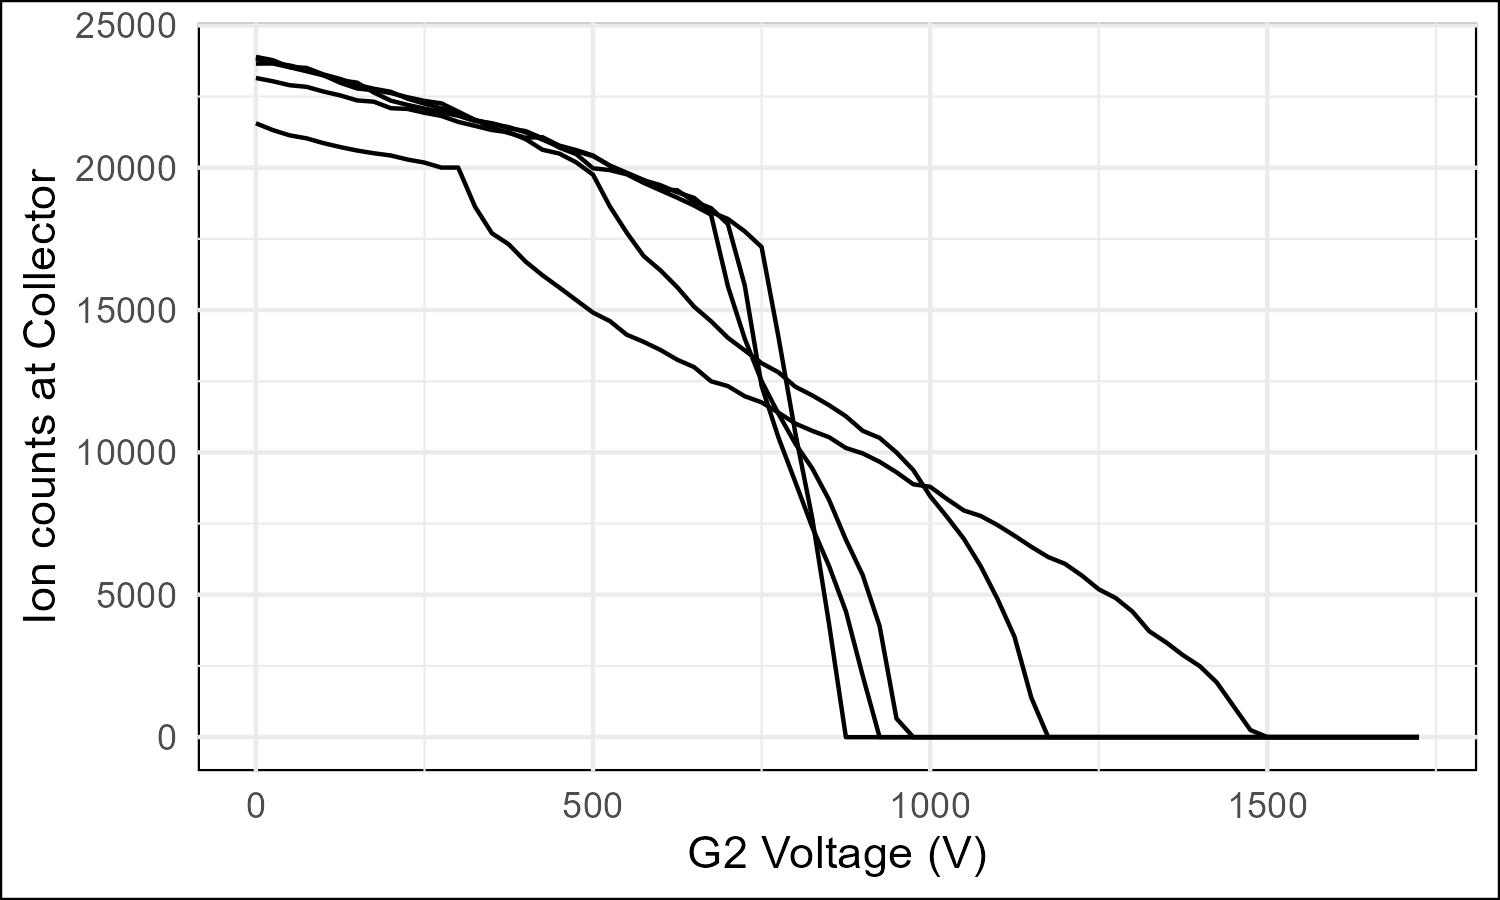
\includegraphics[width=0.45\textwidth]{Figures/IVcurve_FrequencyScan.jpeg}
\caption{Current-voltage characteristic curves where the current is represented by the ion count collected at the collector position. The curves correspond to frequency settings from 2~Mhz to 27.12~MHz. The pressure was set to 0.5~Pa. }
\label{fig:IVcurve_FrequencyScan}
\end{figure}

\begin{figure}[htbp]
\centering
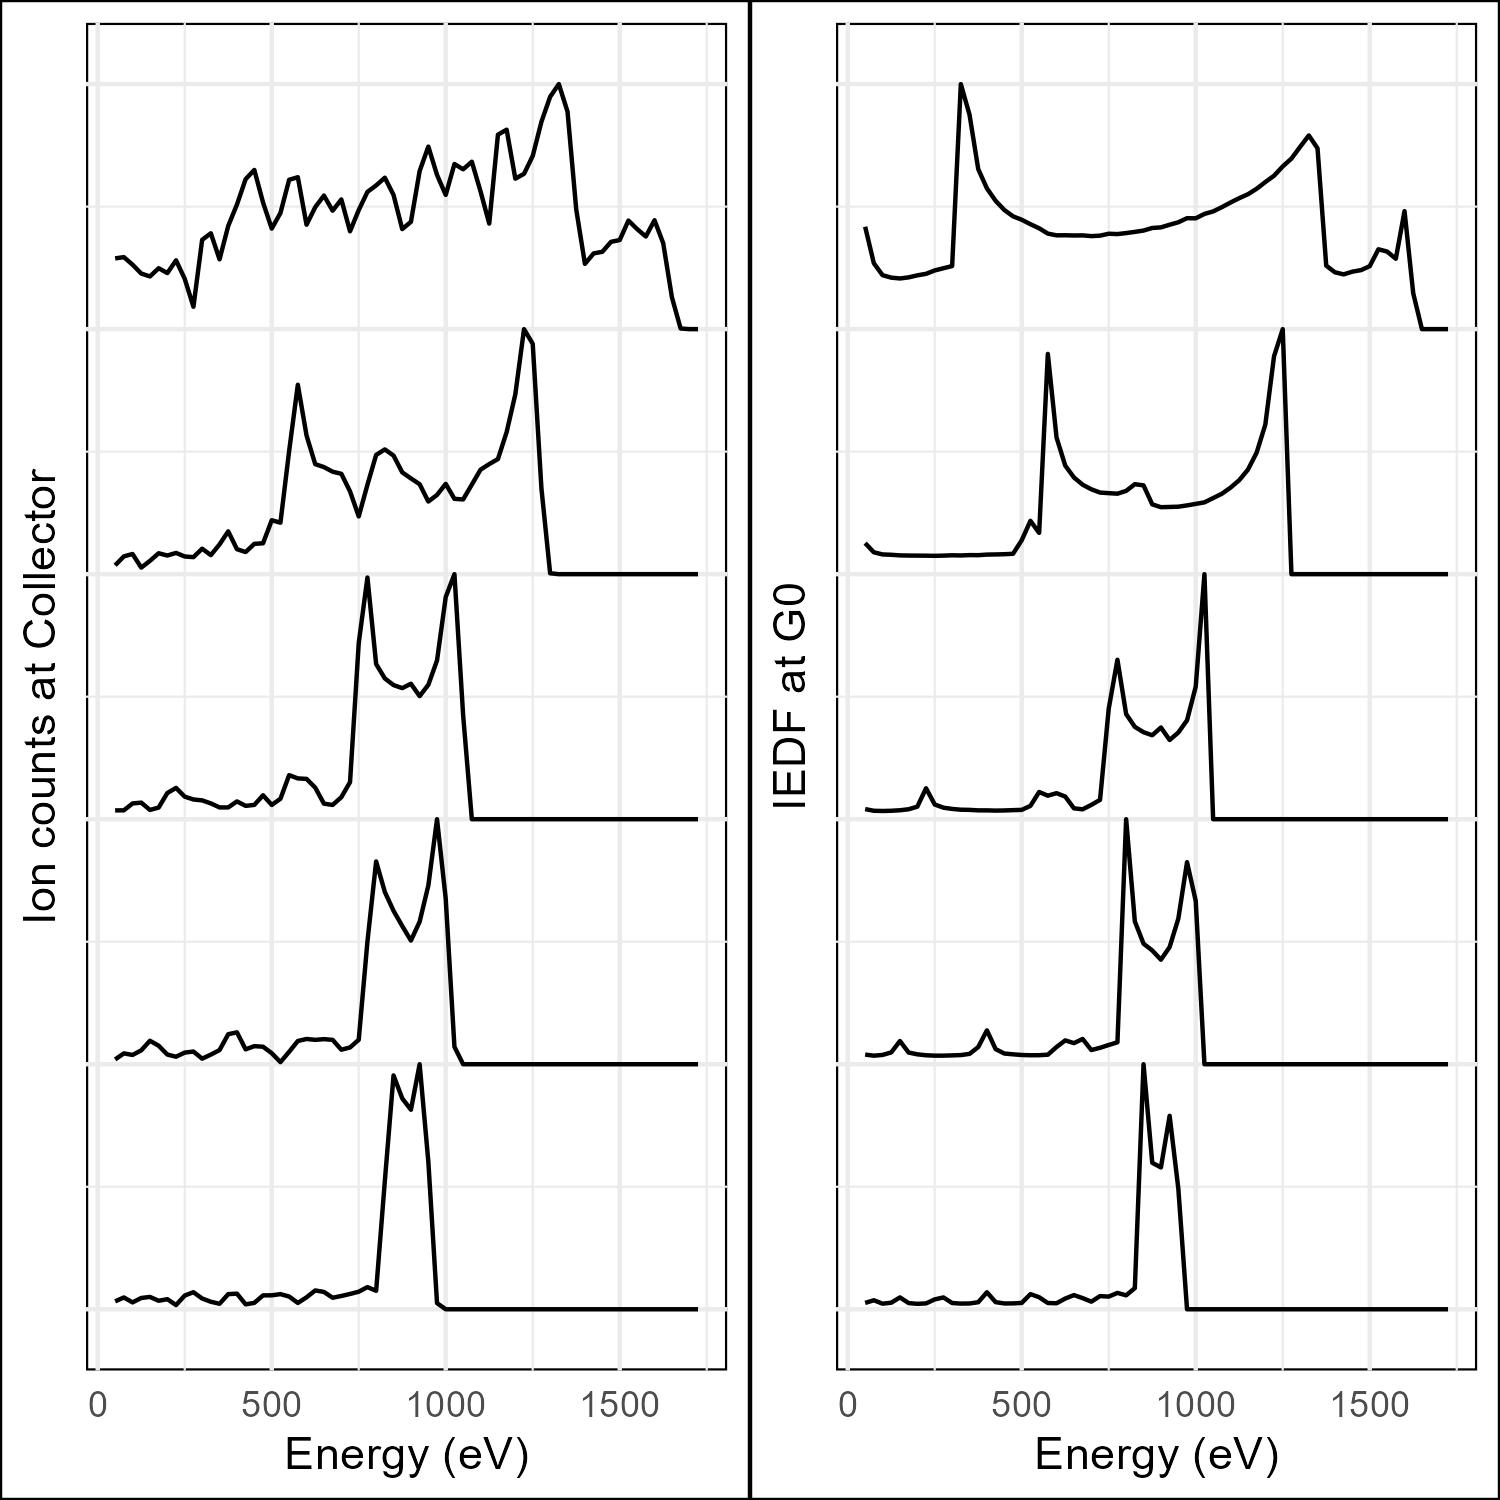
\includegraphics[width=0.45\textwidth]{Figures/FrequencyScan.jpeg}
\caption{Ion energy distribution functions. Left: First derivative of the current-voltage characteristic curves of Figure~\ref{fig:IVcurve}. Right: Plot of the ion energy distribution as recorded in the simulation at G$_0$, before ion transport through the RFEA. Both set of curves are normalized. The curves from top to bottom correspond to frequency settings from 2~MHz to 27.12~MHz. The pressure was set to 0.5~Pa.}
\label{fig:FrequencyScan}
\end{figure}




\subsection{Pressure transparency estimate}
The ion current to the collector in an RFEA can be attenuated mainly by two factors: a geometrical transparency factor, and a collisional transparency factor.  

First, each grid in the analyzer has a open area which can be used to estimate a geometrical transparency. Typically, the open area is 50~\%. The geometrical transparency is influenced by variations in the dimensions of grids openings, the number of openings in each grid, the alignment between grids and lensing effects due to the electric field distortion around the grid surface. As discussed in the description section, we can assign a geometrical transparency to every grid. The geometrical transparency (P$_g$) is the fraction of ions that may reach the collector where the impediment is only due to geometrical effects.  

Second, even though the spacing between grids is typically small (i.e., in the order of 100s of $\mu$m) ion collisions with neutrals may occur even at low pressures. As described before, the dominant collision process is charge exchange which effectively takes away all the energy gained by the ion in the sheath. Therefore, any collisions before the discriminator G$_2$ or at a distance after the discriminator grid where the space potential is below the potential of the collector would prevent said ion from reaching the collector~\cite{Baloniak2010}. The collisional transparency (P$_c$) is the fraction of ions that may reach the collector where the impediment is only due to ion collisions with the neutral background gas. 

The total ion current attenuation is the product of the two transparency factors.
\begin{equation}
P_{\text{total}} = P_\text{g} + P_\text{c}
\end{equation}

The pressure scan results can be used to estimate the collisional transparency. Using a similar procedure as that done experimentally, we can compare the number of ions reaching C with those passing through G$_0$ with no ion discrimination, i.e., G$_2 =0$. In the simulation, for each G$_2$ voltage setting 25000 ion trajectories were simulated. Therefore, the number of ions reaching the collector when G$_2$ is set to null divided by the 25000 is the collisional transparency. Figure~\ref{fig:CollisionalTransparency} shows the estimated collisional transparency from the pressure scan data. The relationship seems to be linear. We need to verify that the ion transit time is much shorter than the models 1~$\mu$s. 

\begin{figure}[htbp]
\centering
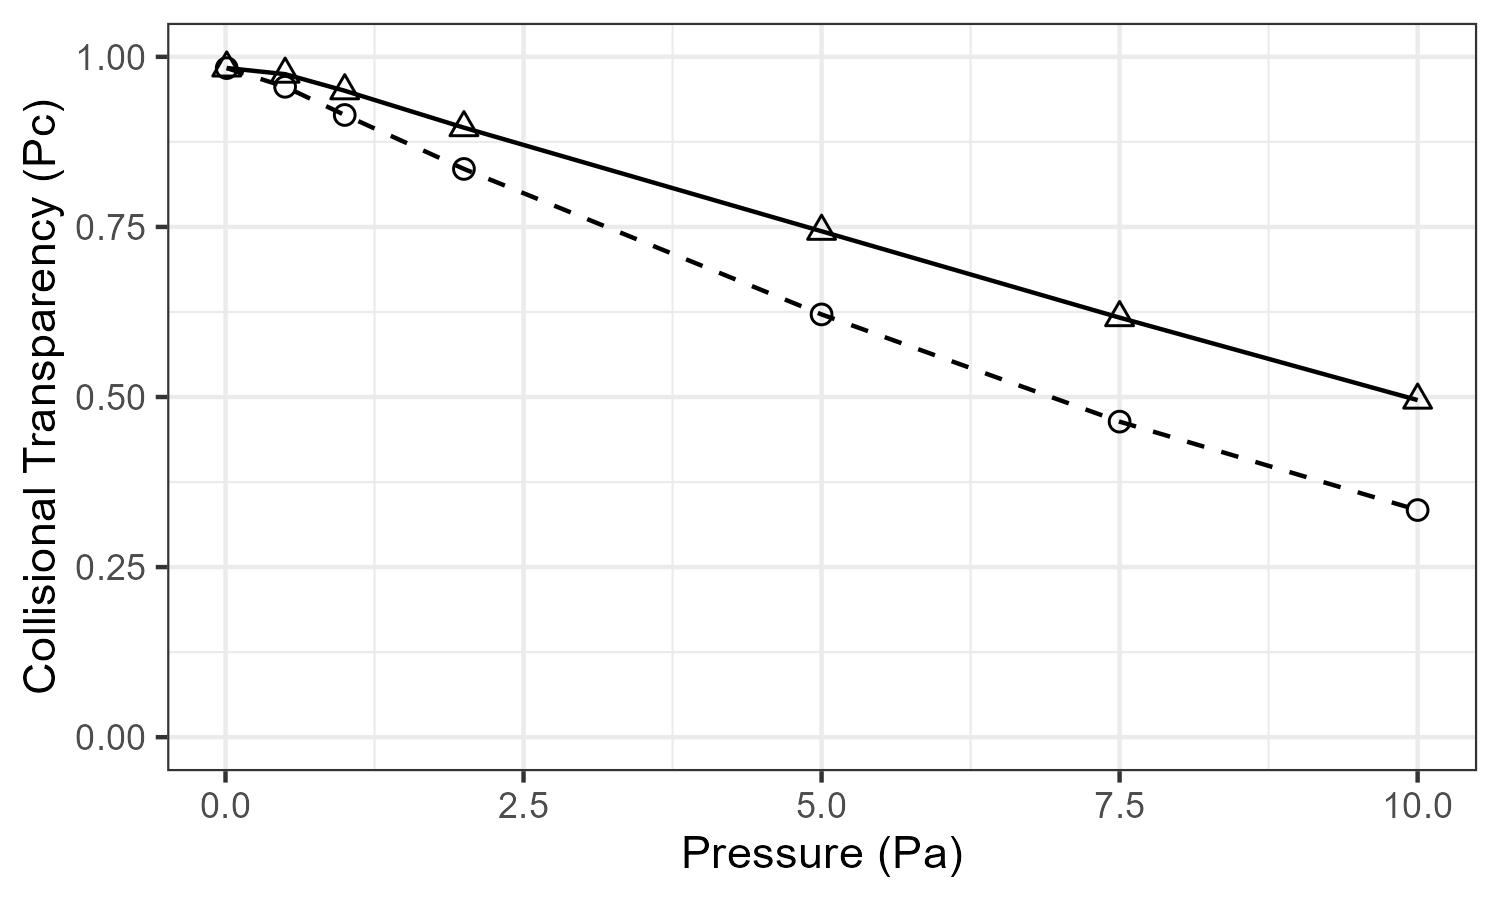
\includegraphics[width=0.45\textwidth]{Figures/CollisionalTransparency.jpeg}
\caption{Estimated collisional transparency (P$_g$) as a function of argon neutral gas pressure.}
\label{fig:CollisionalTransparency}
\end{figure}

We can udpate this graph by doing a collisional transparency scan (i.e., set a scan with only one value of G2 =0 at different pressures, 13.56 MHz) and using a different button stack (for example 2772).